\chapter{Introduction} \label{chap:c1_IntroductionAOI}

\section{Motivation} \label{sec:Motivation} %arbel

The following story is a true story about the NSA - the US intelligence agency
and their classified internal journal named "Cryptographic Spectrum".
In the US, there is a law called ``The Freedom of Information Act'' (FOIA). This lawy states that in general, any person can ask for an access to government documents.
So, in 2007, a lawyer named Michael Ravnitzky, went ahead and asked for the table of
contents of all the articles in the NSA journal. The NSA tried postponing his request for several years, but finally granted him what he asked, along with a censorship on some classified titles. Then, after receiving that, he simply continued asking for the other classified titles!

One article that was published in the journal, named ``Tempest: A Signal Problem'',
tells us about something that happened in the years of World War II. In those years,
there were some significant scientific developments, one of them being digital wireless
communication. People were able to send messages from one side of the world to the other, using digital signals. However, the US army that actually used this way of communication was not willing to be intercepted by the enemy so in order to protect those transmissions, it had to encrypt them. 

At the end of the encryption process, we get a ciphertext, which can be
transmitted without any concern. The obstacle which prevents attackers from
decrypting the ciphertext and discover the key is the algorithm which has been
implemented very well. Let us assume we have a weak computer to perform the
encryption, given that in the years of World War II there were no resistors, no
iterative circuits - what can the adversary do to find the key?

The adversary can build a machine which does the decryption - insert the
ciphertext into the machine and try all the keys (brute force). But\ldots how do
you know which key is the correct one? Simple, there is a logic to the plaintext.
It could be a chat in English, a weather broadcast, even an executable - in general, it is
something you can check the syntax for, so with a very high probability, if you get
an output that starts with ``Heil Hitler'' -  the key you used to decrypt the
ciphertext is the correct key. We need to remember that the encryption machine
was not very complex in those years, and to keep the secure messages safe, they
had to find a way to protect their ciphertexts. The solution to that issue is a
one-time pad.

One-time pad, also called Vernam Cipher, is a simple and powerful encryption
system. The idea behind this technique is that the length of the key is the same
length as the plain text, and to encrypt you just add them together - if we use
digital bits we use XOR, and if we use letters we define an addition operation.
It's called a one-time pad because you can use your pre-shared key only once.

Why does this one-time pad protect from brute force attacks? Because $plaintext
\oplus key = ciphertext$ and $ciphertext \oplus key = plaintext$, meaning we can
take the ciphertext and any plaintext we want, XOR them together, and get the
corresponding random key. In a very secure encryption technique, like AES-256,
there are \(2^{256}\) possible keys and with a ciphertext which is 1MB, we have
\(2^{8000000}\) possible keys, but if we don't know the key there are
\(2^{256}\) random plaintext, and maybe just one of them is the real one. The
one-time pad has been proven to be completely secure by Claude Shannon, and
there is no way to break it.

Back to the years of World War II, to use one-time pad those days, they used
machine which called \textbf{AN/FGQ-1 mixer}~\cite{cryptoMix} as can be seen in
\Cref{fig:Mixer}.

\begin{figure}[!ht]
    \centering
    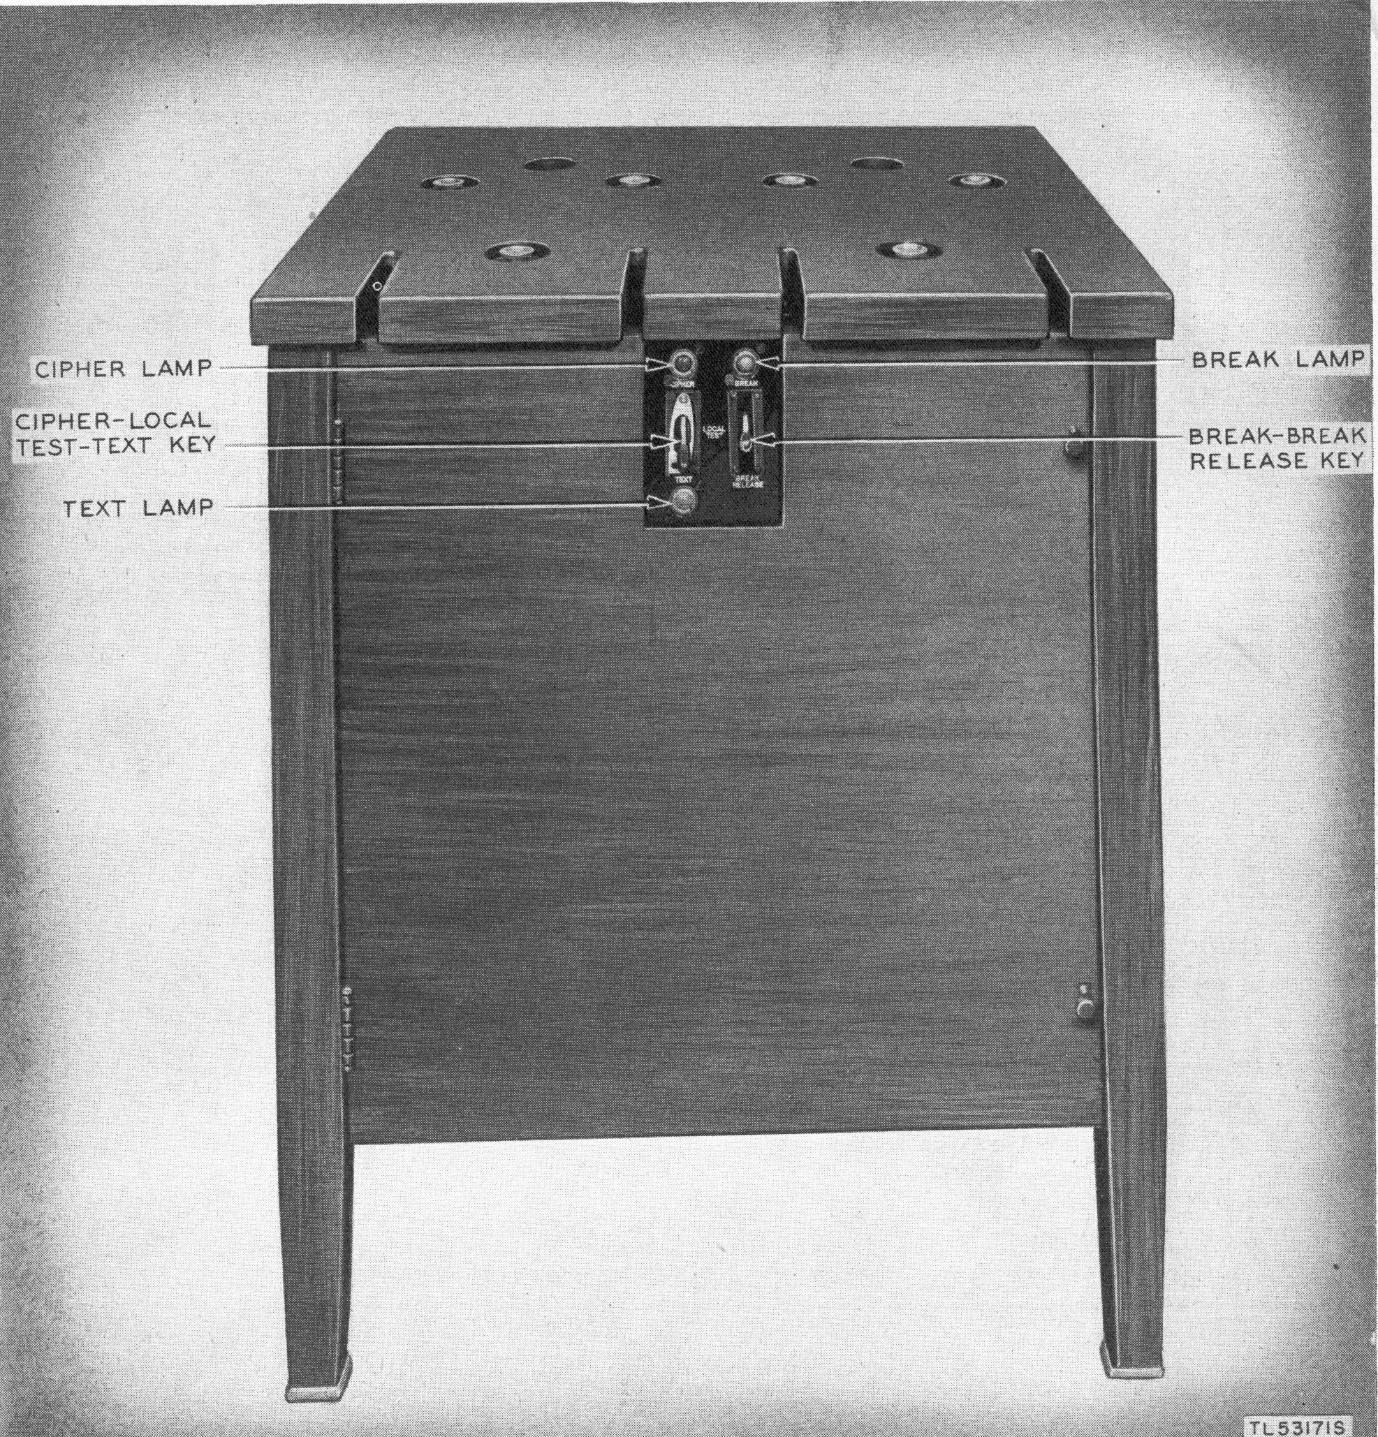
\includegraphics[width=0.8\textwidth]{images/ch1_Intro/MIxer.jpg}
    \caption{\textbf{AN/FGQ-1 Mixer}. Two-way teletypewriter repeater and mixer equipment enclosed in a wooden Table-type cabinet.} \label{fig:Mixer}
\end{figure}

This machine is a kind of a box, and next to the box, was seated a wireless
operator with a typewriter. The tape that came out from the typewriter was
with holes that spooled into the box together with another piece of tape, which
was the key. Inside the box there were little lights that lit through the holes, and
little punches which would punch holes in the third piece of tape. The XOR result of
the plain text and the key was the output of one operation of the machine. Then, the wireless operator fed the ciphertext into the digital radio to transmit.

Is the machine classified? If the system is designed right - you can tell the
adversary whatever you want except for the secret key, and the system will
remain secure.

So, these machines were used during the war, until they broke down, and at the
time that happened, they have been sent to the Bell Labs (which produced the
machines). The engineers who tried to repair one of the machines that sat in a room,
and on the other side of the room, there was an \textbf{Oscilloscope}. 

An Oscilloscope is like babies monitor - just for signals. You connect the
Oscilloscope to an electric circuit, and there is a line that rising every time
there is a difference in voltage. \Cref{fig:Oscillo} demonstrates such a setup.
This Oscilloscope was not connected to the mixer, it was just laying at the other
side of the room, connected to some other test equipment. The engineers
discovered that every time this mixer entered the digit into the tape, they would
get a pulse at the Oscilloscope. This is bcause that when you send a current into an electric monitor, the current is moving through the conductor and electromagnetic current is being generated. The Oscilloscope has little wires, and the electromagnetic
waves can travel through those wires. As a result, we have a transmit antenna and
a receive antenna, so the Oscilloscope measures the holes (the ciphertext) in
the tape. Another possible explanation is that when the punches punch a hole in the
tape, it consumes so much current that the voltage in the room drops a little,
and then the lines in the Oscilloscope, without being connected to anything,
just ``jump''.

\begin{figure}
    \centering
    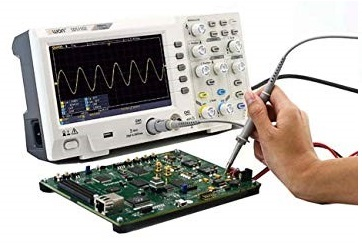
\includegraphics[width=0.8\textwidth]{images/ch1_Intro/oscilloscope.jpg}
    \caption{\textbf{Oscilloscope}. An electronic test instrument which graphically displays varying signal voltages as a function of time.}
    \label{fig:Oscillo}
\end{figure}

The engineers discovered~\cite{NSAsecret} that the top-secret information inside
this machine was being transmitted over the air. The process the engineers were
supposed to do is called responsible disclosure, meaning to report a bug. Like
good engineers, they told the Secret Service people about this bug, but they
did not take their diagnosis seriously. So what did they do? The Bell labs were
located next to the US Secret Service office, so they set up an antenna and
they listened for an hour for radio transmissions that the Secret Service got in
their office, and they gave the Secret Service their ``top-secrets'' analyzed
messages.

Obviously, the US Secret Service realized that the reported attack was not
esoteric, and they asked for a solution from the engineers. The solution of Bell
labs was to modify the mixers - to surround them in a wire cage which will
absorb the radiation coming out from the machine, to put a shield on the
machine (to make sure the power consumption is not affecting the outside), and
to make sure that people are not getting close to the machine more than 30
meters. The Secret Service people decided to accept just the distance solution
and not the filtering/shielding/isolation solutions, because of the high
expenses and time that would cost to modify all the machines during wartime.

In 1954, the Soviet Union published a tender to build military phones. They were
very specific about protecting the phones by shielding them and making sure they
do not generate too much radiation. In addition, they were also publishing strict tenders for other things like engines, turbines, etc. In fact, this is an evidence that in those years, the Soviet Union actually knew about the ``bug'' in the machine.
In conclusion, a one-time pad is the most secure cipher known, but from
the story above, we can see it was broken. So, what was broken? \textbf{The
implementation}.

\begin{figure}[!ht]
    \centering
    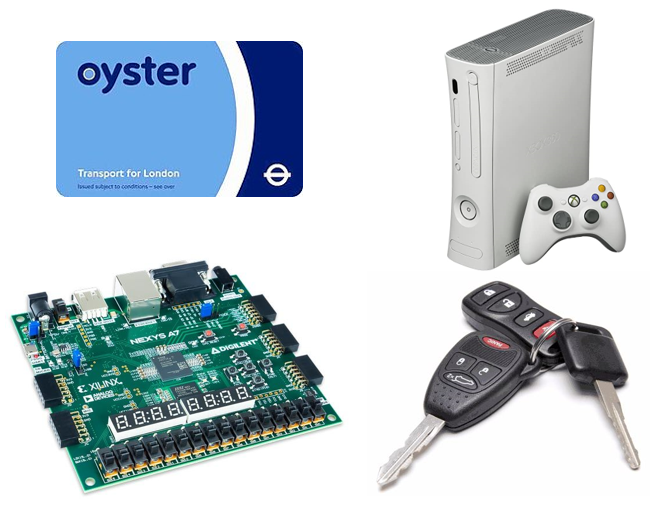
\includegraphics[width=0.8\textwidth]{images/ch1_Intro/modern_systems.png}
    \caption{\textbf{Modern Systems}. A few modern systems that are vulnerable to implementation attacks.}
    \label{fig:Modern Systems}
\end{figure}

Here are a couple of \textbf{Modern Systems} which will break using attacks on their
implementation:

\begin{itemize}
    \item \textbf{Xbox 360}: Xbox is a PC that plays nothing but games, it is
    very cheap and you pay for the games. Attackers, obviously, want to crack
    the Xbox - to play games for free, to watch movies on the device or to run
    Linux. In Xbox there are some integrity checks, and one of the checks was
    done by a command called ``memory compare'' ~\cite{memcmp}, so you would
    calculate the integrity check over whatever software it supposes to run and
    you would have it stored in the secure memory, and then you would try to
    compare using these 2 values. This command leaks the length of the number of
    correct bytes before the first incorrect byte, so if you compare 2 blocks
    and the first bit is different - the response will be fast, and if the
    blocks identical until the very last bit - it would take a longer. This is
    one of the things that was enough to break the machine. 
    \item \textbf{Oyster Card}: it is a computer without power supply and inside
    this computer there are stored values. Attackers could attack this card to
    take the train for free. There are a lot of ways to attack the implantation
    of that card~\cite{garcia2008dismantling, courtois2008algebraic}.
    \item \textbf{Car Keys}~: Car hacking has become more commonplace in recent years, due to the increased integration with electronic systems that include the car’s own lock system.
    With keyless entry systems, it uses wireless or radio signals to unlock the car.
    These signals can in turn be intercepted and used to break into the car and even start it.
    One such technique is called SARA or Signal Amplification Relay Attack. \cite{relayAttack}
    \item \textbf{FPGA}~\cite{fpga}: a piece of hardware which is a very
    versatile, meaning we can find it many kinds of hardware - routers, audio
    equipment, spaceships, etc. the FPGA has a firmware installed inside, and if
    you want to copy some designs you need to find the firmware. The firmware is
    encrypted, but a bunch of Germans researches
    discovered~\cite{moradi2011vulnerability} that if you measure the power
    consumption of the FPGA while it is encrypting the firmware - you can find
    out what is the key.
\end{itemize}

When we implement an algorithm without being careful, we can be exposed to
implementation attacks. To protect ourselves against those attacks, we must protect the implementation, but as we saw at World War II, this countermeasure has a price. It makes the system more expensive, and heavier.

\section{System Implementation} \label{sec:SystemImpl}

The simplest form of a computational system is a device which gets input, makes
a computation and finally produces an output as can be seen in
\Cref{fig:SecDev1}. We assume that our system contains a secret, which is not
revealed to anyone before, during and after the computation process. 

\begin{figure}[!ht]
    \centering
    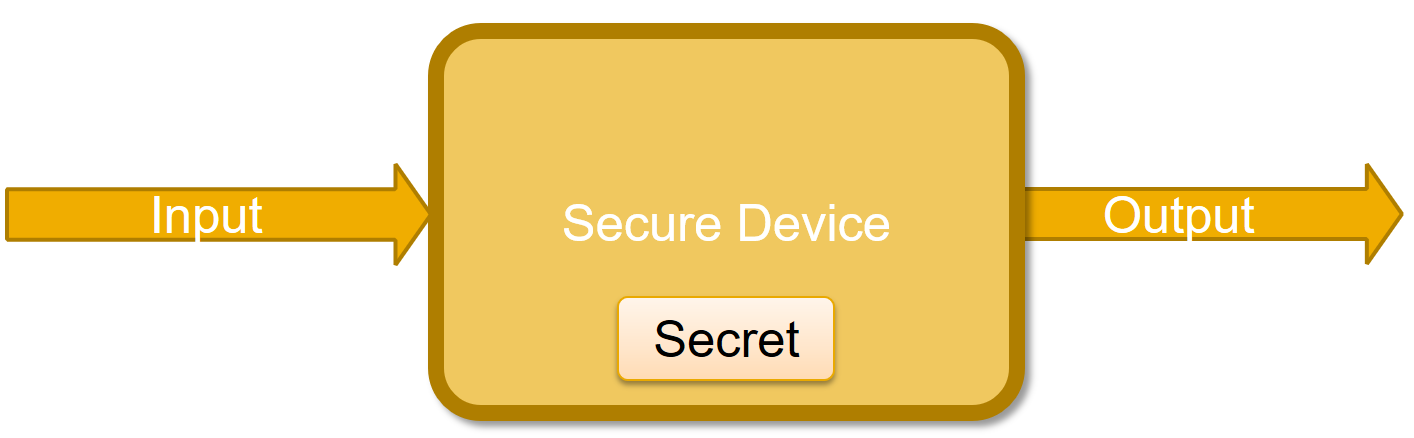
\includegraphics[width=0.8\textwidth]{images/ch1_Intro/Secure_device1.png}
    \caption{\textbf{Simplest Model}. The device make a computation using the secret and the input, and outputs the result.} \label{fig:SecDev1}
\end{figure}

But, if that all what the ``system'' has, it is not a system, it is just an
algorithm. What turns an algorithm to be a system? It is the implementation!

Think about ATM - very simple device without cryptography. The input is our
credit card and a 4-digits PIN code, the output is money. If we do not know the
PIN code we can go over the all possible combinations of 4-digits code (brute
force), and finally find the correct PIN. Unfortunately, we have a limit of 3
trials until the card is being shredded. What an attacker can do?

As an output, and besides the money, we have also some additional outputs which
have been produced by the implementation of the physical system. Those
additional outputs are called ``Side Channels'' and they are in fact outputs that the
system designer did not intend to produce. Those outputs are demonstrated in
\Cref{fig:SecDev2}

\begin{figure}[!ht]
    \centering
    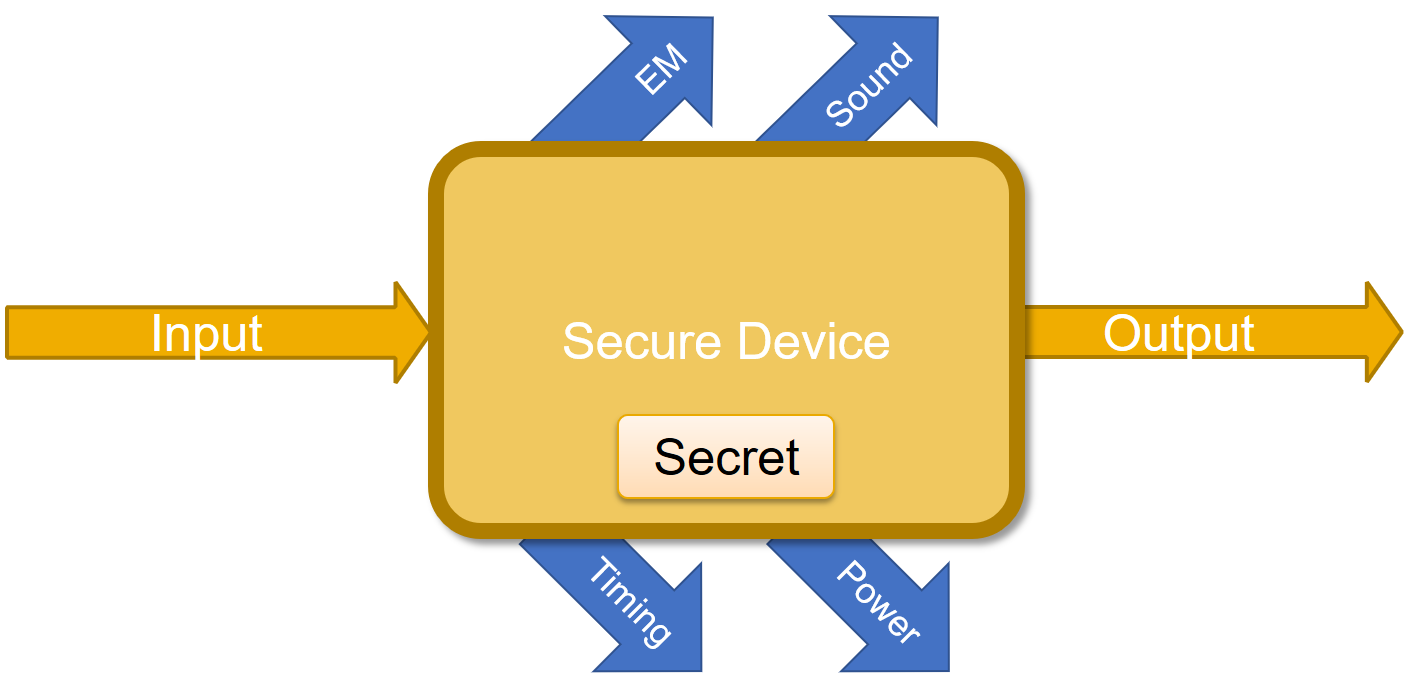
\includegraphics[width=0.8\textwidth]{images/ch1_Intro/Secure_device2.png}
    \caption{\textbf{Side Channels of the System}. Caused by the implementation of the system}
    \label{fig:SecDev2}
\end{figure}

For example, we can measure the time it takes to complete an operation,
measure electromagnetic radiation, listen to the sound of the device while an operation is being completed, measure power, etc. These are \textbf{Passive Attacks} - meaning that we are letting the device to do its ``stuff'' while we are just listening.

There are also \textbf{Active Attacks} - also called fault attacks which try to
break the device under test in a way that it will be ``just a little bit broken''.
It can be done by turning it off in the middle of a calculation, changing its clock, etc. 
As a result, we might not get the actual secret, but we will get some kind of errors that can tell us a lot about the secret. 

\begin{figure}[!ht]
    \centering
    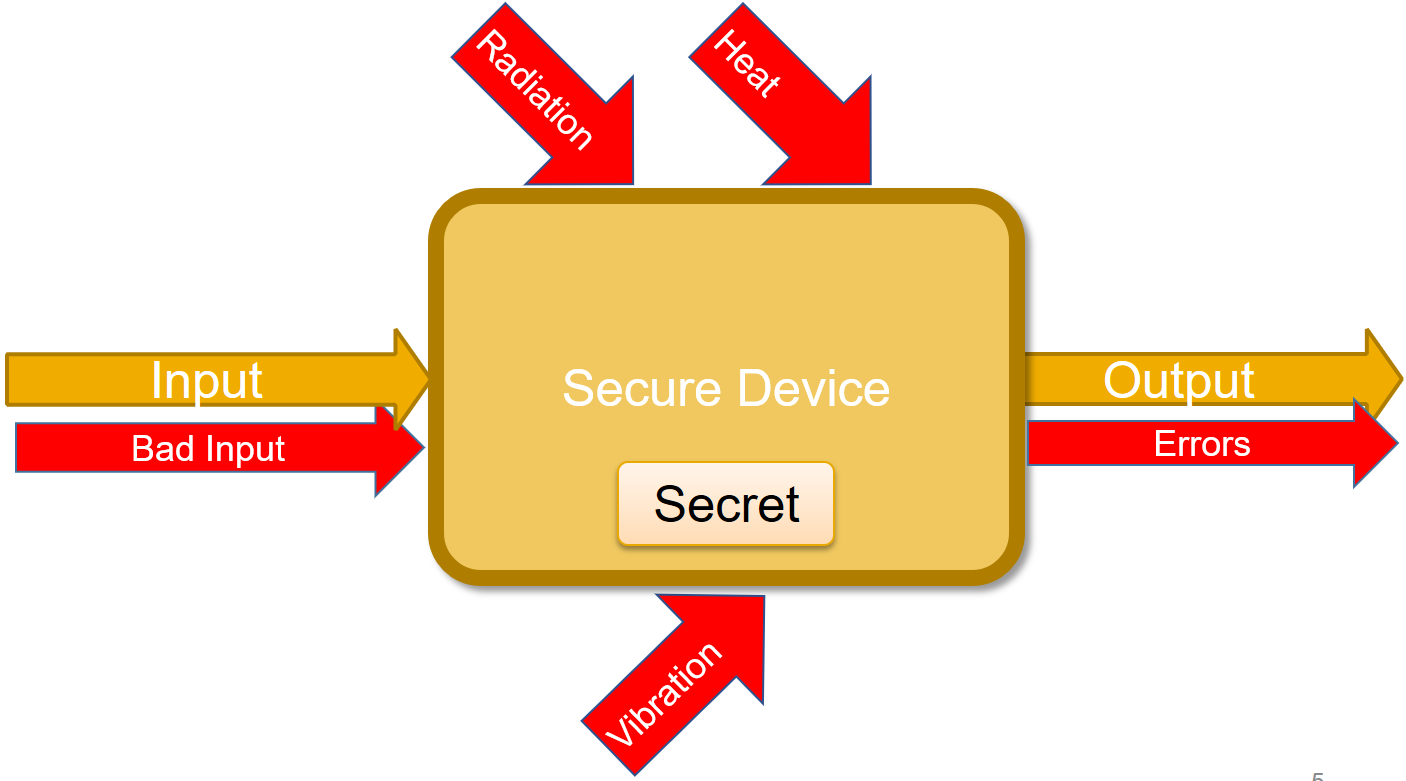
\includegraphics[width=0.8\textwidth]{images/ch1_Intro/Secure_device3.png}
    \caption{\textbf{Fault Attacks}. Manipulating the device through side channels}
    \label{fig:SecDev3}
\end{figure}

\section{Security of a System} \label{sec:SystemSecurity}

When we can say that a system is secured? Usually, we define a system as a
``secured system'' if the system maintains three aspects of information security,
known as the CIA~\cite{cia} triad:

\begin{itemize}
    \item \textbf{Confidentiality} - when you are interacting with a system, you
    only get what you wanted to get. For instance, when I check my test grade,
    I will get my grade and not my friend's grade. If I eavesdropped a conversation for example, it will no longer be confidential.
    \item \textbf{Integrity} - all the data in the system is correct. A possible
    attack could be that one side of the communication will accept a message
    they are not supposed to accept. If I managed to manipulate a bank withdrawal, or jailbreak a device, its integrity would be compromised.
    \item \textbf{Availability} - the system must work in a reasonable time. A
    possible attack could be a Denial of Service (DOS).
\end{itemize}

In \Cref{fig:CIA} the relation between those aspects is demonstrated as the
Triangle of Information Security.

We do not have to use cryptography to secure our system. For example, if someone
goes to some event without invitation, there is a security to prevent him from
getting in.

An \textbf{Algorithm} is a process or set of rules to be followed in
calculations or other problem-solving operations. An example of an algorithm is
GCD/Extended GCD. An algorithm is secure when it is implementing the CIA triad
mentioned above. A \textbf{Protocol} is when you need to get something done, for
example, AES -  the input is a 128-bit key and a 16-bytes plaintext (in case of
different amount of bytes we can use block cipher like CBC), and the output is a ciphertext.

\begin{figure}
    \centering
    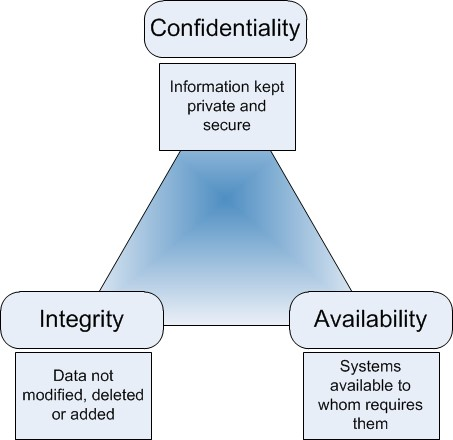
\includegraphics[width=0.5\textwidth]{images/ch1_Intro/cia.jpg}
    \caption{\textbf{CIA Triangle}. The classic model for information security. Defines three objectives of security: maintaining confidentiality, integrity, and availability. Each objective addresses a different aspect of providing protection for information.}
    \label{fig:CIA}
\end{figure}

The millionaire problem~\cite{lin2005efficient} is a classic problem by Yao and
which introduce the question of whether two millionaires can learn who is richer, 
without revealing to one another how much money they each have. 
One possible solution, they could invite a poor man, tell him the secret of
how much money each one has, and the poor man will announce who is richer.  

Cryptographically Secure Algorithms and Protocols:
\begin{itemize}
    \item \textbf{Encryption and Decryption} - Public key-RSA, Symmetric key-AES
    \item \textbf{Signing and verification} - must be an asymmetric key. There
    are 2 parties - signing party and verifying party, who gets the public key.
    The difference between signing and decryption is when one side sends a
    signed message it comes with a signature, and when one side decrypts a
    message it is sending only the ciphertext.
    \item \textbf{Key Exchange} - Diffie Hellman algorithm.
    \item \textbf{Hashing and HMACs} - a hash is a function that gets a long
    input (of arbitrary length) and outputs a fixed size output. A hash
    function is secure when it is difficult to find collisions in it, i.e 2 messages with
    the same hash. HMAC is a hash with a key - when you change the key, the hash
    is also changed.
    \item \textbf{Multiparty Computation} - secure protocols for auctions, votings, etc.
    \item \textbf{Cryptocurrency} - Bitcoin for example.
\end{itemize}

Secure Architectures without cryptography:
\begin{itemize}
    \item \textbf{Secure Policies} - like access control to a military base, for  instance.
    \item \textbf{User Separation and Sandboxing} - a program is divided into
    parts which are limited to the specific privileges they require in order to perform a
    specific task.
    \item \textbf{Virtual Memory} - an application has a view of the memory, and we
    can take to pointer and point to some parts of the memory. We will get our
    old memory (which we are allowed) or the app will crash due to access to
    invalid memory space. In theory, we cannot get another user's memory.
\end{itemize}

\section{Constructing and Using a Threat Model} \label{sec:BreakImpl}

What is the main advantage we have as attackers which allows us to break
implementations that are secure in theory? 
The main advantage is that we have more inputs and outputs which translates into side channels and leakage, so together it means that we can break a completely secure algorithm. 
But when is an algorithm's implementation secure? CIA triad holds, but the thing that is missing here is the \textbf{story}, i.e. what are we allowing the attacker to do with the system?
The more power we give the attacker, the less impressive the attack becomes. 

Let us have a look at a little system where the assumptions were broken:

\begin{figure}[!ht]
    \centering
    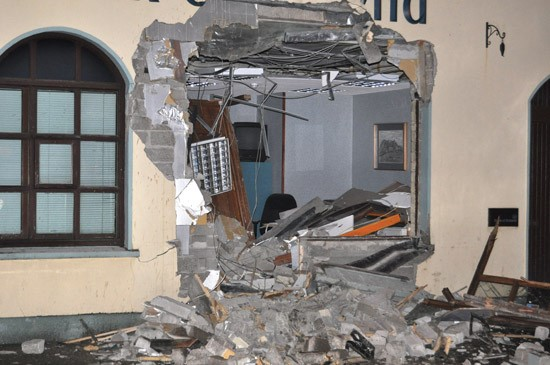
\includegraphics[width=0.8\textwidth]{images/ch1_Intro/Bank.jpg}
    \caption{\textbf{ATM theft.} The thieves simply ripped the machine out of the wall.}
    \label{fig:Bank}
\end{figure}

\Cref{fig:Bank} presents a wall of a bank in Ireland, on which an ATM was
constructed. As we know, the ATMs are very secure systems - they have
encryption, they check our ID very carefully and if we make any mistake they
shred the card. What just happened, is that the ATM was stolen from the wall of a bank
by thieves which took a vehicle and smashed it through the wall. They then loaded the ATM on their track, and left the vehicle to prevent the police from chasing them. 
We can learn from this story, that although the ATM was secure, the threat model was wrong.

The most important thing about the threat model is the story. Once we have the story, we can find out what are the different properties. We specify them as follows:

\begin{itemize}
    \item \textbf{Victim Assets} - what does the victim have that I can steal? 
        \begin{itemize}
            \item \textbf{Cryptographic secretes (keys)} -  the keys are short,
            and when one key is stolen, - the attack has succeeded. There are
            two kinds of keys, long term, and short term.
                \begin{itemize}
                    \item \textbf{Long Term Key } - the private key that
                    identifies a server. If the key is stolen, it will be possible
                    to sign malware as a software update.
                    \item \textbf{Short Term Key} - a key that is generated during
                    a session and is initialized from the long-term key. If this key gets stolen  it is possible to decode all the messages in the current session and modify/inject them.
                \end{itemize}
                Notice that if the long-term key is stolen, it does not mean the short-term key is stolen.
            \item \textbf{State secrets} - for example, ASLR or configuration of
            a system. If someone can find out the addresses of functions in the
            memory of a victim, he can write exploits. 
            \item \textbf{Human secrets} - things which the users do not want to
            reveal like passwords, medical condition, etc.
        \end{itemize}
    \item \textbf{Attacker Capabilities} - what can the attacker do?
        \begin{itemize}
            \item \textbf{Off-path} - the attacker is sitting somewhere in the
            world - cannot observe or communicate with you, but he can attack you
            somehow. 
            \item \textbf{Passive Man in the Middle} - attacker who can see the
            victim communication with the server, but cannot communicate with the victim directly.
            \item \textbf{Active Man in the Middle} - an attacker who can
            interact with the server and can do replay attacks.
            \item \textbf{Physical Access} - an attacker who has physical access
            to the victim. For example, removing or unplugging or melting stuff
            in the system.
        \end{itemize}
        An important thing we need to consider when we are talking about
        attacker capabilities is the other defenses we must protect our system with, like
 guards or cameras. Another thing is the scale of the attack, meaning how many systems we can attack at once. If the attack is physical, it is probably just one system. If the attacker attacks from an android application, he might attack all the phones in the world.
    \item \textbf{Attacker Objectives} - who are the attackers? What do they
    want?
        \begin{itemize}
            \item \textbf{Stealing stuff} - the attacker might want to steal
            your secrets.
            \item \textbf{Duplicating stuff} - for example, the attacker can buy
            one smart TV card, and generate a thousand duplicates from this card
            to sell them. 
            \item \textbf{Forging stuff} - the attacker creates something new,
            driver licenses for instance.
            \item \textbf{Corrupting stuff} - the attacker breaks something and
            decommissioned the system.
        \end{itemize}
\end{itemize}

Of course, the more limits we put on the attacker, the more and more
impressive the attack becomes.

\section{Related Work} \label{sec:RelatedWork}
The whole topic of Attacks on implimitation has been widly reaserched,
and side channels attacks have been found on many varius types of implantation.
Here are a few interesting such types of side channels attacks
 and examples for actoual attacks on those topics:
\begin{itemize}
    \item \textbf{Audio-based attacks} - for example, ultrasonic beacons and acoustic cryptanalysis. 
    a type of side-channel attack that exploits sounds emitted by computers or other devices.
    Most of the modern acoustic audio-based attacks focus on the sounds produced by computer keyboards and internal computer components,
    but historically it has also been applied to impact printers and electromechanical deciphering machines.
    here are a few examples of real-life acoustic attacks: 
    \begin{itemize}
        \item \textbf{1} In 2004, Dmitri Asonov and Rakesh Agrawal of the IBM Almaden Research Center announced that computer keyboards and keypads used on telephones and automated teller machines (ATMs) are vulnerable to attacks based on the sounds produced by different keys.
         Their attack employed a neural network to recognize the key being pressed.
         By analyzing recorded sounds, they were able to recover the text of data being entered.
         These techniques allow an attacker using covert listening devices to obtain passwords, passphrases, personal identification numbers (PINs), and other information entered via keyboards.
         In 2005, a group of UC Berkeley researchers performed a number of practical experiments demonstrating the validity of this kind of threat.
        \item \textbf{2} A new technique discovered by a research team at \textbf{Israel's Ben-Gurion University Cybersecurity Research Center} 
        allows data to be extracted using a computer's speakers and headphones. 
        Forbes published a report stating that researchers found a way to see information being displayed, by using a microphone, with 96.5 percent accuracy.
    \end{itemize}
    \item \textbf{Differential fault analysis} those attacks take multiple traces of two sets of data, then computes the difference of the average of these traces.
    If the difference is close to zero, then the two sets are not correlated, and if the p-value (typically ≥ 0.05) is higher, correlation can be assumed to be possible.
    An example of an attack that was achieved by this is cracking the difficult-to-solve 128-bit AES. 
    Using differential fault analysis it was shown that the key can be broken into 16 bytes, where each byte can be solved individually.
    Testing each byte requires only 28, or 256 attempts, which means it would only take 16 x 256 or 4,096 attempts to be able to decipher the entire encryption key. 
    \item \textbf{Data remanence} Data remanence is the residual representation of digital data that remains even after attempts have been made to remove or erase the data.
    This residue may result from data being left intact by a nominal file deletion operation, by reformatting of storage media that does not remove data previously written to the media,
    or through physical properties of the storage media that allow previously written data to be recovered.
    Data remanence may make inadvertent disclosure of sensitive information possible should the storage media be released into an uncontrolled environment (e.g., thrown in the trash or lost)
    an example of an attack that is using data romance is cold boots wich steals sensitive cryptographic materials like cryptographic keys by Keeping DRAMs at lower room temperature,
    say -50 degrees C, and making it hard for the Dram to preserve his data properly.
    more details on this attack can be found here \href{https://resources.infosecinstitute.com/cold-boot-attack/#gref}{cold-boot-attack}.
    \item \textbf{Optical attacks} these attacks range from the relatively simple (eavesdropping on a monitor via reflections) through to complex (communicating with an infected device via LED blinks). 
    An article of optical attack utilizing the photonic side-channel against a public-key of common implementations of RSA \href{https://www.eng.tau.ac.il/~yash/ieee-host-2017.pdf}{optical side-channel against a public-key of RSA}.
\end{itemize}

In addition to those attacks, there are even more side channels attacks research and new weaknesses are discovered every time.
More of such attacks like Specter, RowHummer, and many more will be described widely in this course.

\subsection{Research Highlights}
\title{A Note on the Confinement Problem}
\maketitle
The paper\cite{lampson1973note} discusses the meaning and implications of confining a problem during its execution.
Multiple examples are presented to describe the problem and necessary conditions are stated and justified.\\\\
We are already familiar with the need of protection systems to safeguard the data from unauthorized access or modification and programs from unauthorized execution. This requires creating a controlled environment where another, perhaps untrustworthy program could be run safely and was solved prior.\\\\
Terminology - The customer wants to ensure that the service cannot read or modify any data which he did not explicitly grant access to.\\\\
Even after we prevented all unauthorized access the service may be still able to injure the customer, this can be achieved by leaking the input data that the customer gives it. The service might leak data which the customer regards as confidential and generally there will be no indication that the security of data has been compromised. From now, the problem of constraining a service will be called the confinement problem. We would like to characterize this problem precisely and describe methods to block some of the possible escape paths for data from confinement.\\\\
Our main goal is to confine an arbitrary program. The program may not be able to work as usual when it is under confinement, but it will be unable to leak data.\\\\
Some of the possible leaks might be (1) collecting data and returning it to the owner when called, (2) writing to a permanent file in its owner’s directory, (3) creating a temporary file for the owner to read before the service to complete its work, (4) Using the system’s interprocess communication facility.
After presenting these types of leaks, the paper continues to elaborate about more advanced leaks through covert channels, i.e. channels which are not intended for information transfer.\\\\
The first method is done by exploiting interlocks which prevent files from being open for writing and reading at the same time. The service and its owner can use this to simulate a shared Boolean variable which one program can set and the other can read, for transmitting a single bit. The second method is created by varying the ratio of computing to input/output or paging rate. A concurrently running process can observe the performance of the system and receive this information. \\\\
The channels described above fall into three categories: storage of various kinds, Legitimate communication channels and covert channels.\\\\
The paper then continues to discuss rules for confinement. The first observation is that a confined program must be memoryless. We can now state a rule of total isolation, forcing a confined program to not make any calls to any other programs. However, this rule is impractical. We need to improve this situation. A new confinement rule that we can formulate is transitivity, meaning that if a confined program calls another untrusted program, the called program must also be confined.\\\\
Then, two simple principles are presented. The first one is called masking. This rule states that a confined program must allow the caller to determine its input into the different channels. However, in the case of covert channels, one further point must be made. We need to ensure that the input of a confined program to covert channels conforms to the caller's specifications. This might require slowing the program down, generating spurious disk references etc.

